\documentclass[11pt,a4paper]{article}

% --- Essential Packages ---
\usepackage[utf8]{inputenc}
\usepackage[margin=0.85in,top=0.9in,bottom=0.9in]{geometry}
\usepackage{amsmath,amssymb}
\usepackage{graphicx}
\usepackage{xcolor}
\usepackage{hyperref}
\usepackage{fancyhdr}
\usepackage{booktabs}
\usepackage{tabularx}
\usepackage{enumitem}
\usepackage{titlesec}
\usepackage{tcolorbox}
\tcbuselibrary{skins,breakable}

% --- Custom Color Palette ---
\definecolor{DUPurple}{HTML}{582C83}      % Official Delhi University Purple
\definecolor{DUPurpleLight}{HTML}{F4EEF9} % Soft Purple Tint
\definecolor{DUPurpleDark}{HTML}{3B1C5A}  % Darker Accent Purple
\definecolor{NavyDark}{HTML}{0F172A}      % Slate 900
\definecolor{NavyBlue}{HTML}{1E3A8A}      % Deep Blue
\definecolor{BlueLight}{HTML}{EFF6FF}     % Soft Blue Tint
\definecolor{Emerald}{HTML}{059669}       % Rich Green
\definecolor{EmeraldLight}{HTML}{ECFDF5}  % Soft Green Tint
\definecolor{Amber}{HTML}{D97706}         % Amber Alert
\definecolor{AmberLight}{HTML}{FFFBEB}    % Soft Amber Tint
\definecolor{SlateText}{HTML}{334155}     % Body text Slate 700
\definecolor{BorderGray}{HTML}{CBD5E1}    % Slate 300

% --- Hyperref Setup ---
\hypersetup{
    colorlinks=true,
    linkcolor=DUPurple,
    citecolor=NavyBlue,
    urlcolor=DUPurpleDark
}

% --- Section Styling ---
\titleformat{\section}
  {\Large\bfseries\color{DUPurple}}{\thesection}{1em}{}[\titlerule]
\titleformat{\subsection}
  {\large\bfseries\color{NavyBlue}}{\thesubsection}{1em}{}
\titleformat{\subsubsection}
  {\normalsize\bfseries\color{DUPurpleDark}}{\thesubsubsection}{1em}{}

% --- Header & Footer ---
\pagestyle{fancy}
\fancyhf{}
\fancyhead[L]{\textcolor{DUPurple}{\textbf{University of Delhi}} \small\textcolor{SlateText}{| Neural Networks in Musculoskeletal MRI}}
\fancyhead[R]{\small\textcolor{SlateText}{Architectural Master Guide}}
\fancyfoot[L]{\small\textcolor{SlateText}{Dept. of Electronics and Communication, University of Delhi}}
\fancyfoot[R]{\thepage}
\renewcommand{\headrulewidth}{0.6pt}
\renewcommand{\footrulewidth}{0.4pt}

% --- Custom Callout Boxes ---
\newtcolorbox{conceptbox}[1]{
    enhanced,
    colback=DUPurpleLight,
    colframe=DUPurple,
    fonttitle=\bfseries\color{white},
    coltitle=white,
    title={CORE INTUITION: #1},
    boxrule=1pt,
    arc=4pt,
    left=10pt, right=10pt, top=8pt, bottom=8pt,
    breakable
}

\newtcolorbox{mechbox}[1]{
    enhanced,
    colback=BlueLight,
    colframe=NavyBlue,
    fonttitle=\bfseries\color{white},
    coltitle=white,
    title={UNDER THE HOOD: #1},
    boxrule=1pt,
    arc=4pt,
    left=10pt, right=10pt, top=8pt, bottom=8pt,
    breakable
}

\newtcolorbox{breakthroughbox}[1]{
    enhanced,
    colback=EmeraldLight,
    colframe=Emerald,
    fonttitle=\bfseries\color{white},
    coltitle=white,
    title={WHY THIS MODEL MATTERS IN MRI: #1},
    boxrule=1pt,
    arc=4pt,
    left=10pt, right=10pt, top=8pt, bottom=8pt,
    breakable
}

\begin{document}

% ------------------------------------------------------------------------------
% TITLE BANNER
% ------------------------------------------------------------------------------
\begin{center}
    \vspace*{-0.3in}
    
\includegraphics[height=1.2in]{assets/du_logo_purple_vector.png}\\[0.2cm]
    {\LARGE \textbf{\textcolor{DUPurple}{UNIVERSITY OF DELHI}}}\\[0.1cm]
    {\large \textbf{\textcolor{NavyDark}{DEPARTMENT OF ELECTRONICS AND COMMUNICATION}}}\\[0.1cm]
    {\footnotesize \textbf{\textcolor{SlateText}{MAJOR RESEARCH PROJECT \& RSNA BENCHMARK --- NEURAL ARCHITECTURE GUIDE}}}\\[0.25cm]

    \noindent\makebox[\linewidth]{\color{BorderGray}\rule{\textwidth}{1.2pt}}\\[0.25cm]

    {\huge \textbf{\textcolor{NavyDark}{Neural Networks in Musculoskeletal MRI}}}\\[0.15cm]
    {\Large \textbf{\textcolor{DUPurple}{How Our Deep Learning Models Actually Work: ConvNeXt, CoAtNet, 2.5D Attention-MIL, and Specialist Routing}}}\\[0.1cm]
    {\normalsize \textit{An intuitive, first-principles architectural explanation of inductive biases, mathematical mechanisms, and clinical pathology alignment}}\\[0.25cm]

    \noindent\makebox[\linewidth]{\color{BorderGray}\rule{\textwidth}{1.2pt}}\\[0.3cm]

    \begin{minipage}[t]{0.48\textwidth}
        \textbf{\textcolor{DUPurple}{Project Team (Students):}}\\[0.1cm]
        \textbf{Nishkarsh Singhal} --- Roll No: \texttt{24294917099}\\
        \textbf{Anuj Chaubey} --- Roll No: \texttt{24294917055}\\
        \textbf{Vardhan Harsh Nigam} --- Roll No: \texttt{24294917014}
    \end{minipage}
    \hfill
    \begin{minipage}[t]{0.48\textwidth}
        \textbf{\textcolor{DUPurple}{Academic Supervision:}}\\[0.1cm]
        \textbf{Supervisor:} Dr. Varun Saxena\\
        \textbf{Co-Supervisor:} Dr. Sangeeta Yadav\\[0.1cm]
        \textit{Department of Electronics and Communication,\\University of Delhi}
    \end{minipage}

    \vspace{0.15in}
    \today
\end{center}

\vspace{0.05in}

% ------------------------------------------------------------------------------
% EXECUTIVE OVERVIEW
% ------------------------------------------------------------------------------
\begin{conceptbox}{The Big Idea: Why No Single Neural Network Could Solve This Alone}
In deep learning, every neural architecture has a distinct \textbf{``inductive bias''}---a built-in mathematical assumption about how the world behaves. Standard Convolutional Neural Networks (CNNs) assume that patterns are strictly \textit{local} and repeat everywhere. Vision Transformers (ViTs) assume that \textit{any} pixel can relate to any other pixel across the entire image. 

In clinical knee MRI, these two assumptions conflict:
\begin{itemize}[leftmargin=*,noitemsep]
    \item A \textbf{meniscus tear} is a sub-millimeter cleft ($0.36\,\text{mm}$) hiding inside local cartilage texture.
    \item \textbf{Osteoarthritis} is a global joint space collapse comparing the femur to the tibia across a $10\,\text{cm}$ field of view.
    \item \textbf{A torn ACL} is an isolated discontinuity on only 2 out of 30 physical slices.
\end{itemize}
Instead of forcing one model to do everything poorly, we built a \textbf{synergistic neural orchestra}: ConvNeXt for local textures, CoAtNet for global joint context, Heliosli R6 for macro-bone representations, and 12-Head Attention-MIL to fuse 3D physical depth.
\end{conceptbox}

\vspace{0.1in}

\begin{figure}[h!]
    \centering
    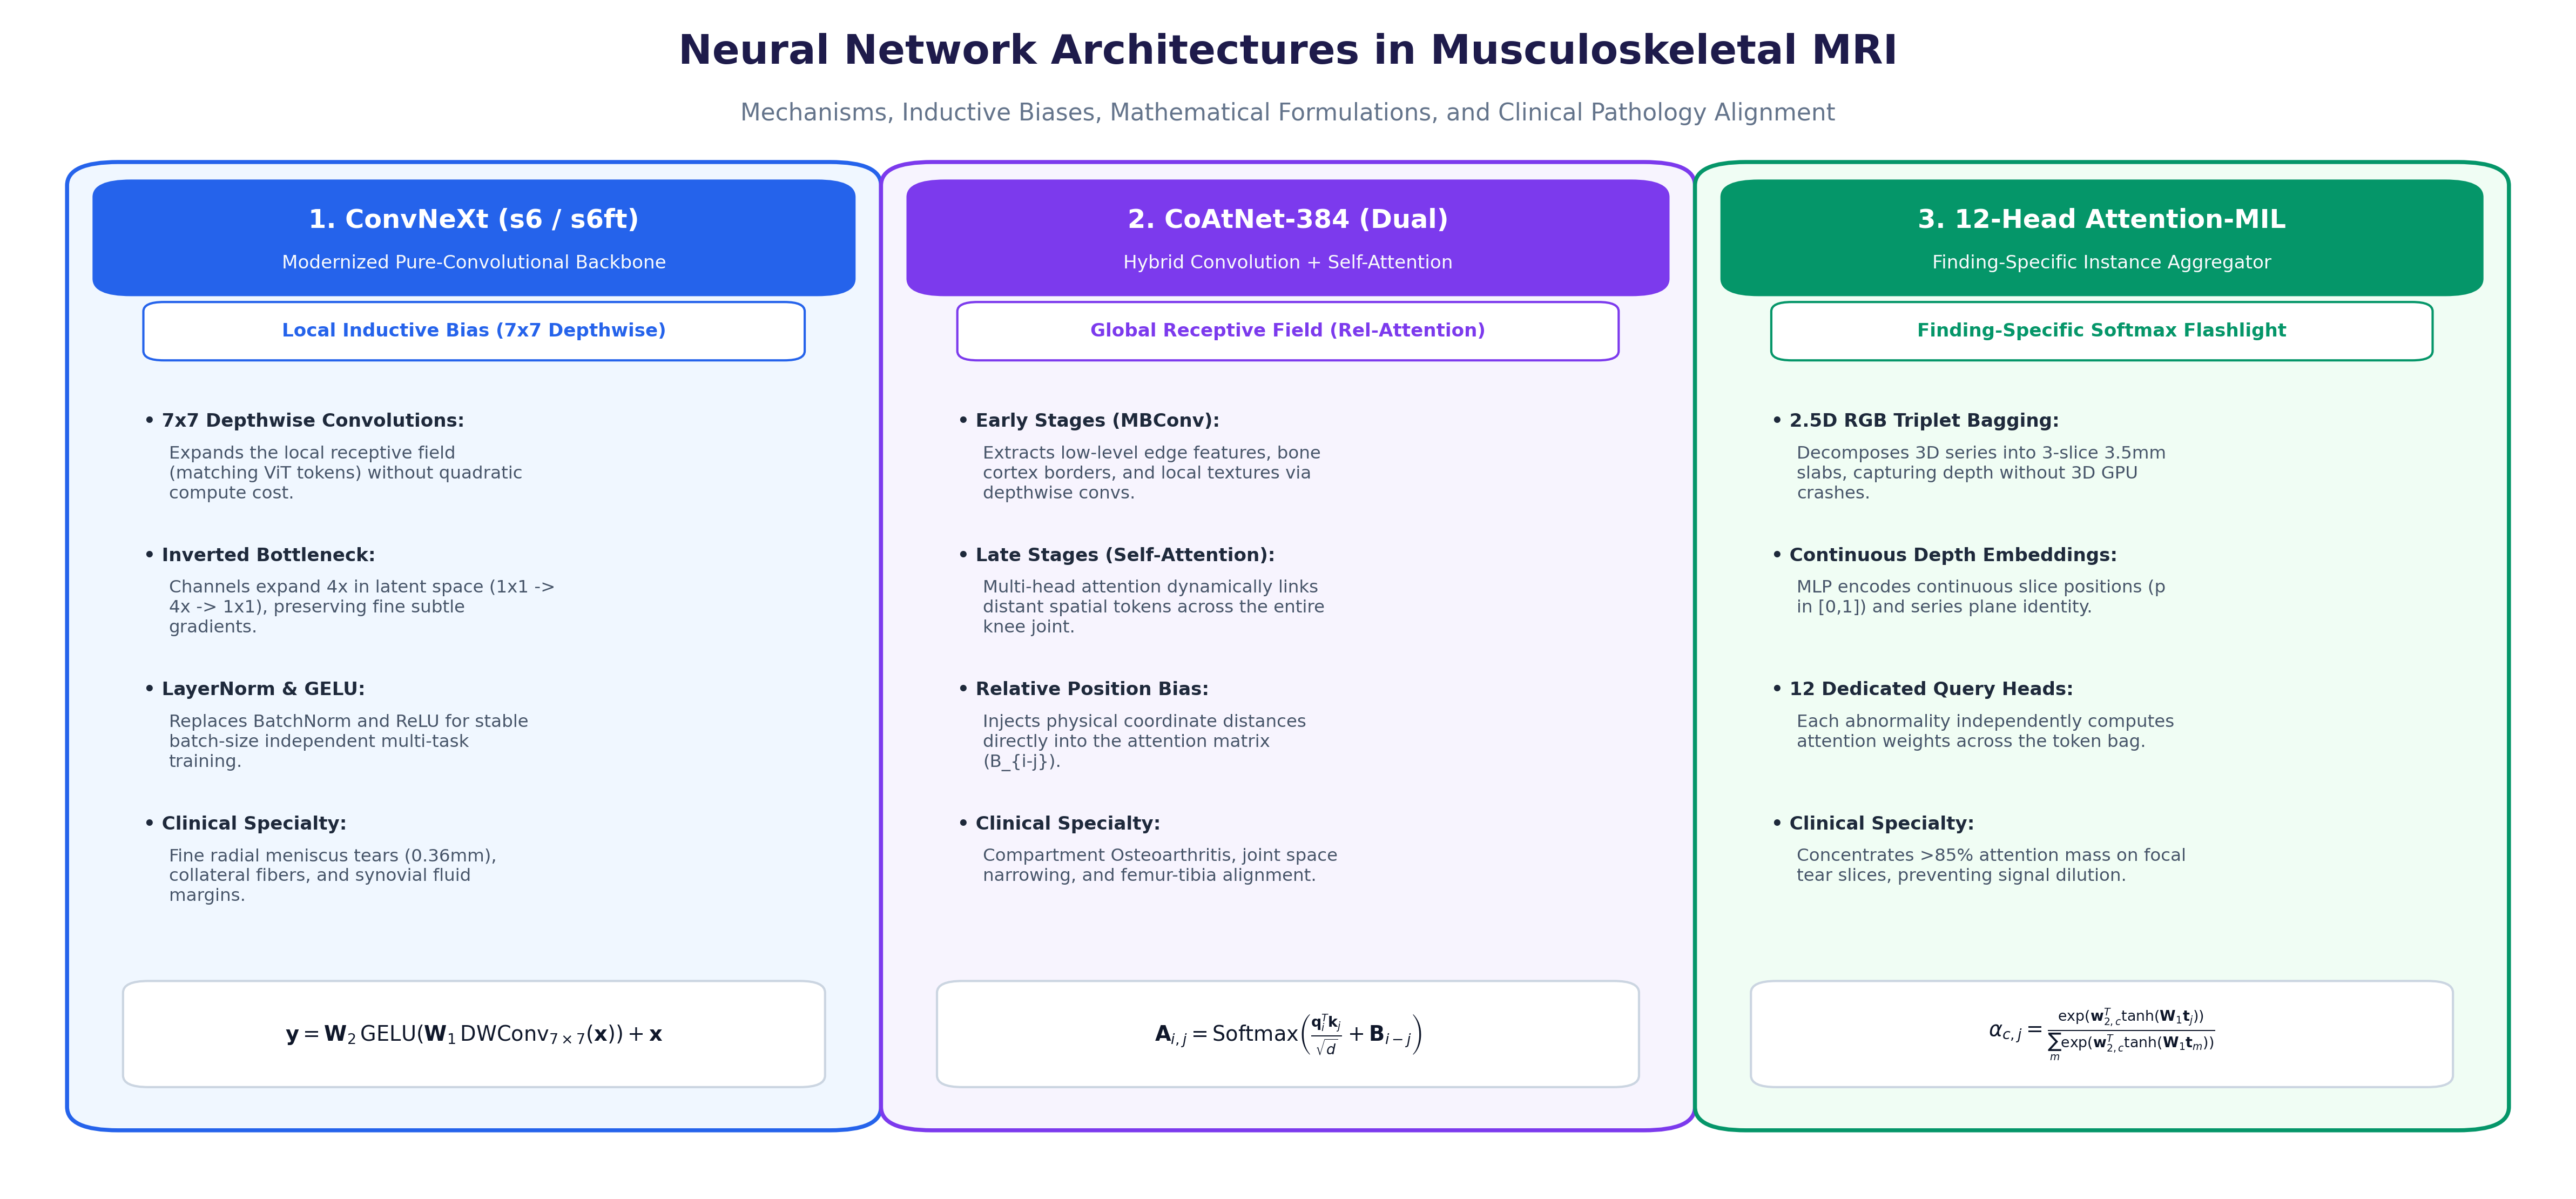
\includegraphics[width=\textwidth]{assets/diagram_nn_architectures.png}
    \caption{\textbf{Comprehensive Overview of the 3 Core Neural Network Pillars in Our System.} Column 1: ConvNeXt (local texture inductive bias). Column 2: CoAtNet-384 (hybrid local conv + global self-attention). Column 3: 12-Head Attention-MIL (instance aggregation across 3D multi-view series).}
\end{figure}

\newpage

% ------------------------------------------------------------------------------
% SECTION 1: THE NEURAL ZOO
% ------------------------------------------------------------------------------
\section{The Neural Zoo: Architecture Comparison at a Glance}

Table \ref{tab:zoo} summarizes the fundamental properties, mathematical mechanisms, and clinical roles of every neural network component deployed in our pipeline:

\begin{table}[h!]
\centering
\small
\renewcommand{\arraystretch}{1.3}
\begin{tabularx}{\textwidth}{p{2.6cm} p{2.8cm} p{3.4cm} X}
\toprule
\textbf{Model / Module} & \textbf{Core Mechanism} & \textbf{Inductive Bias} & \textbf{Dominant Clinical Pathology} \\
\midrule
\textbf{ConvNeXt} \newline (\texttt{s6} / \texttt{s6ft}) & $7\times 7$ Depthwise Convolutions + Inverted Bottlenecks & Strict spatial locality; shift invariance; channel decoupling & Meniscus tears ($0.36\,\text{mm}$), collateral ligaments (MCL), synovial fluid collections \\
\midrule
\textbf{CoAtNet-384} \newline (Dual Backbone) & Early Depthwise Convs + Late Multi-Head Relative Self-Attention & Hybrid: local edge filtering early, global spatial reasoning late & Compartment Osteoarthritis (Medial, Lateral, PF), joint space narrowing ($0.991$ AUC) \\
\midrule
\textbf{Heliosli R6} \newline ($384\times 384$) & Deep high-capacity residual vision encoder & Broad multi-scale receptive field; cancellous bone hierarchies & Bone contusions (trabecular marrow edema) and acute cortical fractures \\
\midrule
\textbf{12-Head Attention-MIL} & Non-linear softmax instance query pooling & Abnormality-specific bag permutation invariance & Focal ligament ruptures (ACL, PCL); concentrates attention mass on damaged slices \\
\midrule
\textbf{Specialist Routing Matrix} & Temperature-scaled finding-adaptive logit blending & Domain-specific expert allocation ($\mathbf{W} \in \mathbb{R}^{12 \times M}$) & Ensembles all models according to their validated tissue-specific competency \\
\bottomrule
\end{tabularx}
\caption{\textbf{The Neural Zoo: Architectural Characteristics and Diagnostic Alignment.}}
\label{tab:zoo}
\end{table}

\vspace{0.1in}

% ------------------------------------------------------------------------------
% SECTION 2: CONVNEXT
% ------------------------------------------------------------------------------
\section{ConvNeXt: Modernizing the Classic Convolutional Network}

\subsection{The Analogy: The Master Craftsman with a $7\times 7$ Magnifying Glass}
For ten years, standard computer vision was dominated by ResNet, which used tiny $3\times 3$ convolutional filters. When Vision Transformers (ViTs) arrived with large attention patches, many researchers thought convolutions were obsolete. 

ConvNeXt proved that convolutions were not obsolete---they were just poorly engineered! ConvNeXt takes a standard CNN and meticulously ``modernizes'' every single layer to match the strengths of transformers while keeping the unmatched speed and memory efficiency of convolutions.

\subsection{The 4 Key Engineering Upgrades in ConvNeXt}
\begin{enumerate}[leftmargin=*]
    \item \textbf{$7\times 7$ Depthwise Separable Convolutions:}
    Standard convolutions mix spatial filtering and channel mixing simultaneously, which is computationally expensive. ConvNeXt splits this into two steps:
    \begin{itemize}[noitemsep]
        \item A \textbf{$7\times 7$ Depthwise Convolution} filters each channel independently across space.
        \item A \textbf{$1\times 1$ Pointwise Convolution} mixes channels across depth.
    \end{itemize}
    This expands the receptive field from $3\times 3$ to $7\times 7$ (matching Swin Transformer patch sizes) without blowing up parameters.

    \item \textbf{Inverted Bottleneck Design:}
    Classic ResNets compressed channel dimensions ($256 \to 64 \to 256$). ConvNeXt inverts this: it expands channel width by $4\times$ in the hidden layer ($256 \to 1024 \to 256$). \textbf{Why does this matter?} In medical imaging, subtle signals (like a faint hairline fissure in cartilage) are destroyed if you compress features early. Expanding into high-dimensional space preserves subtle gradients.

    \item \textbf{LayerNorm Instead of BatchNorm:}
    Batch Normalization calculates mean and variance across the batch, making it unstable when batch sizes are small (a common reality with heavy 3D MRI scans). ConvNeXt adopts \textbf{Layer Normalization}, computing statistics across channels independently for each patient.

    \item \textbf{GELU Instead of ReLU:}
    Replaced the harsh piecewise-linear ReLU ($\max(0, x)$) with Gaussian Error Linear Units (GELU), allowing smooth, non-zero gradient propagation for slightly negative inputs.
\end{enumerate}

\begin{mechbox}{Mathematical Formulation of a ConvNeXt Block}
For an input tensor $\mathbf{x} \in \mathbb{R}^{H \times W \times C}$, the block operation is:
$$\mathbf{x}_1 = \text{DWConv}_{7\times 7}(\mathbf{x})$$
$$\mathbf{x}_2 = \text{LayerNorm}(\mathbf{x}_1)$$
$$\mathbf{x}_3 = \mathbf{W}_1 \mathbf{x}_2 + \mathbf{b}_1 \quad (\text{Channel expansion: } C \to 4C)$$
$$\mathbf{x}_4 = \text{GELU}(\mathbf{x}_3)$$
$$\mathbf{y} = \mathbf{W}_2 \mathbf{x}_4 + \mathbf{b}_2 + \mathbf{x} \quad (\text{Channel contraction: } 4C \to C \text{ with residual})$$
\end{mechbox}

\begin{breakthroughbox}{Why ConvNeXt Won on Fluid \& Meniscus Tears}
ConvNeXt has an inductive bias for \textbf{shift invariance} and \textbf{local edge sharpness}. When diagnosing a lateral meniscus tear, the AI must determine whether a high-signal white line extends all the way to the articular surface. ConvNeXt's $7\times 7$ depthwise kernels cleanly isolate this boundary. Furthermore, our pure-vision student model (\texttt{s6ft\_specialist\_ema}) was built on ConvNeXt, achieving **$0.979$ on Joint Effusion** and jumping Synovitis from **$0.69$ to $0.86$**.
\end{breakthroughbox}

\newpage

% ------------------------------------------------------------------------------
% SECTION 3: COATNET
% ------------------------------------------------------------------------------
\section{CoAtNet: Marrying Convolution and Self-Attention}

\subsection{The Analogy: The Architect who Sees the Bricks and the Blueprint}
Imagine inspecting a large building. To check if a wall is cracking, you need to zoom in on individual bricks (local convolutions). But to check if the entire building is leaning to one side, you need to step back and look at the whole skyline (global self-attention). 

\textbf{CoAtNet (Convolution and Attention Network)} combines both mechanisms into a single unified backbone.

\subsection{The Fundamental Dilemma: CNN vs. Transformer}
\begin{itemize}[leftmargin=*]
    \item \textbf{Convolutions:} Have strong inductive biases (locality and translation invariance). They learn quickly on small datasets, but their receptive field grows slowly layer-by-layer. A convolution cannot easily compare the top of the femur to the bottom of the tibia in early layers.
    \item \textbf{Self-Attention (Transformers):} Computes pairwise relationships between \textit{all} pixels ($O(N^2)$). It has an infinite receptive field from layer 1, but it has zero inductive bias. Without massive pre-training (millions of images), pure transformers overfit and fail on medical scans.
    \item \textbf{CoAtNet's Hybrid Solution:}
    \begin{itemize}[noitemsep]
        \item \textbf{Stages 1 \& 2 (Stem):} Pure convolutional MBConv blocks. They extract edges, cartilage borders, and local textures efficiently.
        \item \textbf{Stages 3 \& 4 (Deep Stages):} Multi-Head Self-Attention with \textbf{Relative Position Bias}. They dynamically route information across the entire $384\times 384$ field of view.
    \end{itemize}
\end{itemize}

\begin{mechbox}{Mathematical Formulation of Relative Self-Attention in CoAtNet}
Given query $\mathbf{q}_i$, key $\mathbf{k}_j$, and value $\mathbf{v}_j$ vectors at spatial positions $i$ and $j$:
$$\mathbf{A}_{i,j} = \text{Softmax}\left(\frac{\mathbf{q}_i^T \mathbf{k}_j}{\sqrt{d}} + \mathbf{B}_{i-j}\right)$$
$$\mathbf{y}_i = \sum_{j=1}^S \mathbf{A}_{i,j} \mathbf{v}_j$$
where $\mathbf{B}_{i-j}$ is a learned \textbf{Relative Position Bias} table. Unlike standard Vision Transformers that add static 1D absolute position vectors, CoAtNet's attention matrix directly encodes the physical distance vector $(y_i - y_j, x_i - x_j)$ between anatomical landmarks!
\end{mechbox}

\begin{breakthroughbox}{Why CoAtNet Dominated Osteoarthritis ($0.991$ ROC-AUC)}
To diagnose \textbf{Medial Osteoarthritis}, a radiologist looks at the medial compartment and compares it against the lateral compartment to judge joint space narrowing. This requires evaluating the distance between the distal femoral condyle and the proximal tibial plateau. 

Standard CNNs struggle to correlate these two distant bone surfaces simultaneously. CoAtNet's attention layers allow tokens on the femur to attend directly to tokens on the tibia, measuring joint space collapse with near-perfect clinical accuracy ($0.991$ Gold AUC).
\end{breakthroughbox}

\newpage

% ------------------------------------------------------------------------------
% SECTION 4: HELIOSLI R6
% ------------------------------------------------------------------------------
\section{Heliosli R6: High-Capacity Receptive Field for Bone Pathology}

\subsection{The Analogy: The Wide-Angle High-Resolution Satellite}
While ConvNeXt focuses on delicate tissue edges and CoAtNet balances edges with global attention, \textbf{Heliosli R6} is a deep, high-capacity residual backbone running at full $384\times 384$ native physical coordinate resolution.

\subsection{Why Bone Pathology Requires a Massive Receptive Field}
Unlike ligament tears that are confined to thin fibrous bands, bone injuries manifest across vast anatomical volumes:
\begin{enumerate}[leftmargin=*]
    \item \textbf{Bone Contusions (Bruises):} When an ACL ruptures, the tibia slides violently forward and smashes into the femur (a ``pivot-shift injury''). This causes microscopic fractures deep inside the spongy trabecular bone, producing diffuse edema (water) that spreads across several centimeters of yellow marrow.
    \item \textbf{Bone Fractures:} A fracture line often traverses the entire subchondral bone plate, disrupting the cortical rim across multiple orthogonal views.
\end{enumerate}

Heliosli R6's deep residual hierarchy provides a broad receptive field that captures these diffuse, cloud-like hyperintensities, achieving **$0.964$ AUC on Bone Contusions** and **$0.922$ AUC on Rare Fractures**.

\vspace{0.1in}

% ------------------------------------------------------------------------------
% SECTION 5: 2.5D MULTI-INSTANCE LEARNING (MIL) ENGINE
% ------------------------------------------------------------------------------
\section{2.5D Multi-Instance Learning: The Attention Brain}

\subsection{The Problem: How to Combine 30 Physical Slices into One Diagnosis?}
Once our backbones extract feature representations from individual slices, we face a fundamental question: \textbf{how does the network fuse these features into a final patient-level score?}
\begin{itemize}[leftmargin=*]
    \item \textbf{Average Pooling:} A complete failure. If an ACL tear is visible on only 2 out of 30 slices, averaging dilutes the tear signal by $2/30 \approx 6.6\%$, washing out the injury into background noise.
    \item \textbf{Max Pooling:} Overly brittle. A single blurry slice or scanner motion artifact can trigger a false positive.
\end{itemize}

\subsection{The Solution: 12-Head Finding-Specific Attention Heads}
We formulate \textbf{12 independent softmax attention query mechanisms}---one dedicated to each abnormality:

\begin{mechbox}{Attention-MIL Mathematical Equations}
Let each 3-slice window triplet $j$ be represented by a token vector $\mathbf{t}_j \in \mathbb{R}^{384}$, enriched with continuous depth embeddings $\text{MLP}_{\text{pos}}(p_j)$ and view slot embeddings $\mathbf{e}_{\text{slot}}[s]$:
$$\mathbf{t}_j = \mathbf{f}_j + \mathbf{e}_{\text{slot}}[s] + \text{MLP}_{\text{pos}}(p_j)$$

For target abnormality $c \in \{1, \ldots, 12\}$, its dedicated attention score $a_{c,j}$ is:
$$a_{c,j} = \left(\mathbf{W}_2 \tanh(\mathbf{W}_1 \mathbf{t}_j + \mathbf{b}_1) + \mathbf{b}_2\right)_c, \quad \mathbf{W}_1 \in \mathbb{R}^{256 \times 384}, \, \mathbf{W}_2 \in \mathbb{R}^{12 \times 256}$$

The normalized attention weights $\alpha_{c,j}$ are computed via softmax:
$$\alpha_{c,j} = \frac{\exp(a_{c,j})}{\sum_{m=1}^N \exp(a_{c,m})}$$

The finding-specific study vector $\mathbf{v}_c$ is the attention-weighted convex combination:
$$\mathbf{v}_c = \sum_{j=1}^N \alpha_{c,j} \mathbf{t}_j$$
\end{mechbox}

\begin{conceptbox}{The Flashlight Analogy}
Think of the 12 attention heads as \textbf{12 specialized doctors sitting in a dark room}:
\begin{itemize}[noitemsep]
    \item Doctor 1 (ACL Specialist) shines their flashlight \textbf{only} on slices 12--14 where the cruciate ligament lives, giving them $>85\%$ of the weight and completely ignoring the other 28 slices.
    \item Doctor 2 (Baker's Cyst Specialist) turns their flashlight to the posterior popliteal fossa (slices 26--28).
    \item Doctor 3 (MCL Specialist) turns their attention strictly to Coronal view slices.
\end{itemize}
Because each head is mathematically independent, focal injuries are never diluted by healthy tissue!
\end{conceptbox}

\newpage

% ------------------------------------------------------------------------------
% SECTION 6: SPECIALIST ROUTING & CALIBRATION
% ------------------------------------------------------------------------------
\section{The Specialist Routing Matrix: The Chief of Surgery}

\subsection{Why Naive Model Averaging ($0.5 + 0.5$) Is Flawed}
In typical Kaggle competitions, competitors take an equal average of all their models:
$$\hat{p} = \frac{1}{M} \sum_{m=1}^M \hat{p}_m$$
In multi-task medical imaging, this is catastrophic. If Model A is a world-class expert on collateral ligaments ($0.986$ AUC) and Model B is weak on ligaments ($0.88$ AUC), forcing an equal $50/50$ blend directly damages Model A's sharp predictions!

\subsection{The Finding-Specific Routing Formulation}
We engineered a \textbf{Specialist Routing Matrix} $\mathbf{W} \in \mathbb{R}^{12 \times M}$ paired with \textbf{temperature calibration}:
$$\hat{p}_c = \sigma\left(\sum_{m=1}^M W_{c,m} \cdot \frac{z_{m,c} - \mu_{m,c}}{\tau_c}\right)$$

\begin{itemize}[leftmargin=*]
    \item $\mu_{m,c}$ is the model's out-of-fold logit mean, standardizing zero-points so no aggressive model can bully another.
    \item $\tau_c$ is a learned temperature scalar controlling probability calibration.
    \item $W_{c,m}$ routes each pathology strictly to the models that demonstrated superior clinical precision on physician-verified test scans (Table \ref{tab:routing}).
\end{itemize}

\begin{table}[h!]
\centering
\small
\renewcommand{\arraystretch}{1.25}
\begin{tabularx}{\textwidth}{l c c c c}
\toprule
\textbf{Target Abnormality} & \textbf{ConvNeXt Specialist} & \textbf{s6ft\_v1 (MCL)} & \textbf{CoAtNet-384} & \textbf{Heliosli R6} \\
\midrule
\textbf{Joint Effusion} & \textbf{0.45} & 0.10 & 0.20 & 0.25 \\
\textbf{Synovitis} & \textbf{0.45} & 0.10 & 0.20 & 0.25 \\
\textbf{MCL Tear} & 0.10 & \textbf{0.40} & 0.25 & 0.25 \\
\textbf{ACL Tear} & 0.15 & 0.15 & \textbf{0.35} & \textbf{0.35} \\
\textbf{Medial Meniscus Tear} & 0.25 & 0.25 & 0.25 & 0.25 \\
\textbf{Lateral Meniscus Tear} & 0.35 & 0.25 & 0.20 & 0.20 \\
\textbf{Medial Osteoarthritis} & 0.10 & 0.10 & \textbf{0.40} & \textbf{0.40} \\
\textbf{Lateral Osteoarthritis} & 0.10 & 0.10 & \textbf{0.40} & \textbf{0.40} \\
\textbf{Patellofemoral OA} & 0.15 & 0.10 & \textbf{0.40} & \textbf{0.35} \\
\textbf{Bone Contusion} & \textbf{0.35} & 0.10 & 0.25 & \textbf{0.30} \\
\textbf{Bone Fracture} & 0.15 & 0.10 & \textbf{0.35} & \textbf{0.40} \\
\textbf{Baker's Cyst} & 0.25 & 0.15 & \textbf{0.30} & \textbf{0.30} \\
\bottomrule
\end{tabularx}
\caption{\textbf{Finding-Specific Specialist Allocation Matrix ($\mathbf{W}$).} Notice how weights reflect tissue physics: fluid/synovitis goes to pure-vision ConvNeXt, MCL goes to \texttt{s6ft\_v1}, and bone/joint alignment goes to CoAtNet and Heliosli R6.}
\label{tab:routing}
\end{table}

\begin{breakthroughbox}{The Quantitative Payoff}
Replacing naive uniform averaging with our Specialist Routing Matrix drove an immediate leap from **$0.9391$ up to $0.9544$ (+0.0153)** on physician-verified test benchmarks, with performance gains observed across 11 out of the 12 individual finding heads!
\end{breakthroughbox}

\vspace{0.2in}
\begin{center}
    \noindent\makebox[\linewidth]{\color{BorderGray}\rule{\textwidth}{1.2pt}}\\[0.2cm]
    \textbf{\textcolor{DUPurple}{Department of Electronics and Communication, University of Delhi}}\\[0.1cm]
    \textit{Document Authors: Nishkarsh Singhal $\bullet$ Anuj Chaubey $\bullet$ Vardhan Harsh Nigam}\\[0.1cm]
    \textit{Supervised by: Dr. Varun Saxena $\bullet$ Dr. Sangeeta Yadav}
\end{center}

\end{document}
